\section{A browsing-data stress test}\label{sec:benchmark}
The empirical question is how much information confusion counts retain for
comparisons supported by an actual browsing matrix. The fixed benchmark contains
\BenchmarkUsers{} pseudonymized users, \BenchmarkDomains{} domains,
\BenchmarkRecords{} user--domain records, and \BenchmarkVisits{} visits.
It is the bundled \texttt{fewlab} extract of the June 2022 YouGov Pulse/RealityMine
panel with Blacklight scanner outcomes. The replication package pins the source
commit and file hashes. Its analytic universe contains domains with recorded
scanner labels; exposure shares use visits within that universe as their
denominator. These recorded outcomes are reference labels for the experiment,
not error-free measures of all tracking activity. The exercise makes no causal
or population-representative claim about demographic differences.

We retain the extract's demographic design matrix: an intercept and indicators
for gender, race, education, and source-coded age groups. Omitted categories are Male, White,
HS or Below, and under 25. For each of seven scanner outcomes, we
calculate all twelve non-intercept least-squares coefficients for both visit
totals and visit shares. Each coefficient is a fixed weighted label sum.
Two scanner columns are counts and are dichotomized at a positive value; the
other five are binary. Complete labels, valid joins, positive visits, and full
column rank are checked before estimation.

Predictions are imposed, rather than produced by a fitted classifier. Within
each true class, we randomly flip the integer part of 1\%, 5\%, or 10\% of the
labels. We then perform two distinct exercises. First, holding those predictions
fixed, Proposition~\ref{prop:bounds} gives the true-coefficient range compatible
with their exact confusion counts. Second, holding the reference labels fixed,
we rearrange the same numbers of false positives and false negatives to minimize
or maximize the predicted coefficient. The latter asks whether two classifiers
with identical confusion matrices can report opposing comparisons. It is a
worst-case sensitivity analysis, not an estimate of likely classifier bias.
Extrema are computed separately for each coefficient; a single error arrangement
need not reverse all comparisons at once.

\begin{table}[htbp]
\centering\small
\caption{What exact confusion counts establish at 1\% imposed error in each true class}
\label{tab:browsing}
\begin{tabular}{lrrr}
\toprule
Scanner outcome & Sign identified & Reversal possible & Median width (pp) \\
\midrule
Advertising trackers & 0/12 & 12/12 & 47.8 \\
Third-party cookies & 0/12 & 12/12 & 52.5 \\
Canvas fingerprinting & 0/12 & 12/12 & 29.5 \\
Session recording & 0/12 & 12/12 & 31.6 \\
Key logging & 0/12 & 12/12 & 21.3 \\
Facebook pixel & 0/12 & 12/12 & 43.6 \\
Google Analytics & 0/12 & 12/12 & 21.6 \\
\bottomrule
\end{tabular}

\par\smallskip
\begin{minipage}{\linewidth}\footnotesize
Each row covers twelve demographic coefficients of visit shares in the fixed
browsing frame. ``Sign identified'' counts bounding intervals excluding zero
for fixed random predictions. ``Reversal possible'' counts coefficients for
which rearranging errors with the same confusion matrix can reverse the
reference coefficient's sign. Median width summarizes identification intervals,
measured in percentage points (pp); these are not sampling intervals. Error
counts are rounded down within each true class. All outcomes, coefficients,
scales, and error fractions are included in the machine-readable results.
\end{minipage}
\end{table}

At the smallest imposed error fraction, none of the \BenchmarkContrasts{}
share-coefficient signs is identified by the full confusion matrix
(Table~\ref{tab:browsing}); all permit a sign reversal by rearranging errors.
The corresponding total coefficients show the same pattern, as do the larger
error fractions. This establishes a limitation of confusion summaries for
this frame. It does not establish that actual classifiers make such adverse
errors. For example, the reference female coefficient for Facebook-pixel visit
share is \FocalTruth{} percentage points. For the fixed random predictions,
its count-compatible interval is $[\FocalLower{},\FocalUpper{}]$ percentage
points. Holding the reference labels fixed instead, moving the same errors
can produce predicted coefficients from \FocalAdverseLower{} to
\FocalAdverseUpper{} percentage points.

\subsection{What an audit recovers}
The audit illustration uses that outcome and coefficient, selected in the
research development plan before inspecting their results. We fix one randomly
constructed prediction vector with 5\% errors in each true class. For budgets
of 250, 1,000, and 2,000 domains, we compare stratified random sampling by
predicted label with a design that first audits the most influential domains
(rank of $|w_j|$) using half the budget. The remaining budget is allocated
proportionally across the predicted-label tail strata and sampled randomly
without replacement. All selection rules use known weights and predictions.

Each design is repeated 1,000 times with fixed labels and predictions. On every
draw, the count projection, direct normal interval, and direct Hoeffding
interval use exactly the same audited labels. All target 95\% coverage; the
first covers all linear contrasts of this outcome simultaneously, whereas the
latter two target the declared coefficient. Hoeffding intervals are intersected
with the logical range given the observed labels. This is a conservative
finite-sample baseline; it is not a comparison against the most efficient
available weighted-audit procedures.

\begin{figure}[htbp]
\centering
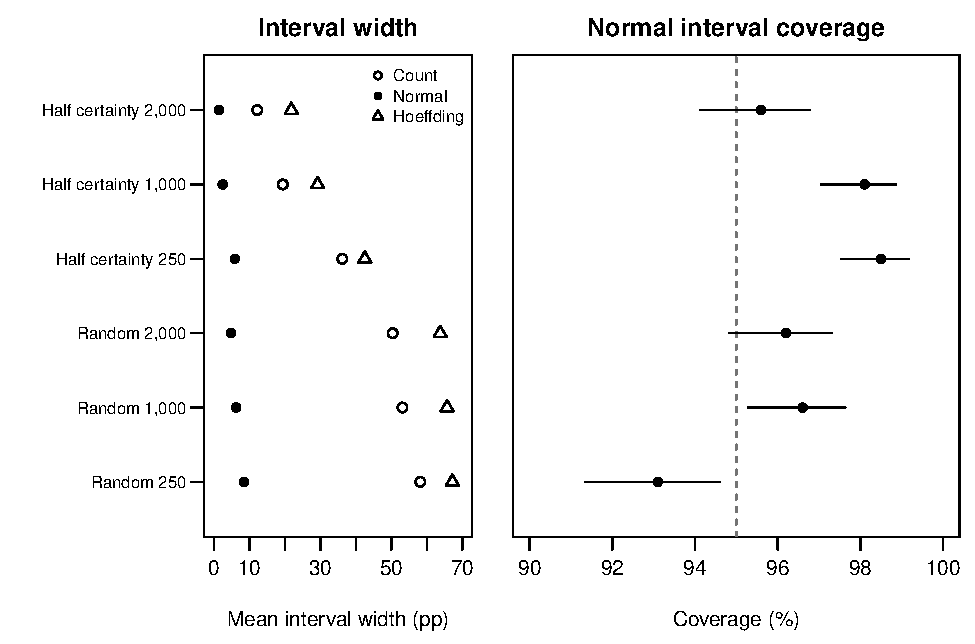
\includegraphics[width=\linewidth]{../figs/audit_comparison.pdf}
\caption{Width and coverage for the Facebook-pixel female share coefficient.
Rows compare audit budgets and designs in the fixed browsing frame. Left:
mean interval width in percentage points over 1,000 audits. Right: normal
interval coverage, with exact 95\% binomial Monte Carlo intervals and a dashed
95\% reference. Count and Hoeffding intervals covered in every simulated draw.
``Half certainty'' audits the largest absolute influences with half the budget.
Count intervals cover all contrasts of this outcome simultaneously; direct
intervals target the declared coefficient. The randomness is domain auditing;
users and predictions are held fixed.}
\label{fig:audit}
\end{figure}

Count projection covered the target in every replication but never excluded
zero. Its intervals were much wider than the approximate normal intervals; the
conservative direct Hoeffding intervals were wider still
(Figure~\ref{fig:audit}). Normal coverage in the smallest entirely
random design was \SmallAuditCoverage{}\%, with Monte Carlo interval
$[\SmallAuditCoverageLower{},\SmallAuditCoverageUpper{}]$\%, below the nominal
level. With 2,000 audited domains and half assigned to the certainty head,
normal coverage was \LargeAuditCoverage{}\% and mean width was
\LargeAuditWidth{} percentage points. These results support retaining the
locations and influences of errors, rather than treating their counts as a
sufficient validation product. They neither establish normal validity for
other outcomes nor an optimal allocation rule. Appendix~\ref{app:audit}
reports every design and method.

\subsection{Finer validation summaries}
Proposition~\ref{prop:sufficient} suggests retaining more information about
influence within a validation table. In a declared follow-up after examining
the initial audit results, we refine predicted-label strata by splitting the
ranks of signed weights into one, five, or twenty-five bins. The resulting
partitions have two, ten, or fifty strata. They use the same fixed prediction
vector and coefficient as the audit illustration. For each partition,
Table~\ref{tab:refinement} separates the identification width if every stratum's
error count were known exactly from the mean confidence-interval width when
those counts must be learned using 1,000 audited domains. The latter allocates
samples proportionally across strata, with at least two observations per
noncensus stratum, and uses 1,000 audit repetitions.

\begin{table}[htbp]
\centering\small
\caption{Refining validation reduces ambiguity but divides the audit budget}
\label{tab:refinement}
\begin{tabular}{rrrr}
\toprule
Strata & Exact-count width (pp) & Audit width (pp) & Coverage (\%) \\
\midrule
2 & 49.7 & 53.2 & 100.0 \\
10 & 34.7 & 47.1 & 100.0 \\
50 & 21.8 & 48.2 & 100.0 \\
\bottomrule
\end{tabular}

\par\smallskip
\begin{minipage}{\linewidth}\footnotesize
Facebook-pixel female share coefficient, fixed reference labels and imposed
predictions. Rank bins of signed influence cross predicted labels. Exact-count
width conditions on the population count in every stratum; audit width averages
95\% count-projection intervals over 1,000 domain samples of size 1,000, with
Bonferroni allocation across strata. Widths are percentage points. Coverage is
empirical; the exact binomial Monte Carlo intervals accompany the results.
No design certified the coefficient's sign.
\end{minipage}
\end{table}

Finer summaries reduce identification ambiguity, as the proposition predicts.
But the narrowest audit intervals among these partitions use ten strata, not
fifty. Learning more stratum counts from a fixed audit budget and protecting
their joint coverage offsets part of the gain. This comparison demonstrates
both a constructive use of the characterization and its practical constraint:
validation strata should preserve relevant weight differences without making
each count too imprecise. It does not select an optimal partition.
